\documentclass[11pt,a4paper]{article}

\usepackage[utf8]{inputenc}
\usepackage[T1]{fontenc}
\usepackage[margin=2cm]{geometry}
\usepackage{graphicx, booktabs, amsmath, hyperref, float, adjustbox, caption, xcolor}
\hypersetup{colorlinks=true, linkcolor=blue, urlcolor=blue}
\graphicspath{{../figures/}}

\title{Learning Descriptive Statistics with Hantavirus Data \\
\large A Step-by-Step Journey Through Distribution Analysis}
\author{}
\date{}

\begin{document}
\maketitle
\thispagestyle{empty}

\section{Introduction}

This document follows my process of applying descriptive statistics concepts learned from a
textbook to a real-world dataset -- as a practice project to learn and improve.
Along the way I share findings, mistakes made, and how they were corrected.

\subsection{Data Source}
Data is from Kaggle: \texttt{https://www.kaggle.com/datasets/zkskhurram/hantavirus-andes-virus-global-epidemiology}

\textbf{Disclaimer:} This is a historical Kaggle dataset on hantavirus epidemiology, \textbf{not} the 2025 outbreak data. This project focuses on learning descriptive statistics, not on current events.

Six datasets covering:
\begin{itemize}
\item \textbf{Clinical:} 7538 patient records (incubation, hospital stay, ICU, severity, outcome)
\item \textbf{Environmental:} 896 location-quarters (temperature, rainfall, rodent abundance, biome)
\item \textbf{Country-Yearly:} 939 country-year observations (confirmed cases, deaths, CFR)
\item Outbreaks, virus strains, monthly trends
\end{itemize}

The data was already well-prepared. No further cleaning was needed beyond noting that
missing symptom data was structural -- each syndrome (HPS vs HFRS) uses a different
symptom checklist, so no imputation was required.

\subsection{Project Structure}

\subsection{Project Structure}
\begin{verbatim}
hanta_project/
  scripts/         Python scripts (01_, D1_, D2_, ..., E1_, F_)
  figures/         All output plots (PDF + PNG)
  explanations/    Per-step documentation
  tables/          LaTeX summary tables
  report/          This report
\end{verbatim}

All scripts use \texttt{np.random.seed(42)} for reproducibility.
Key dependencies: pandas, numpy, scipy, matplotlib, seaborn.

\subsection{Concepts Applied}
Box plots, violin plots, histograms, ECDF, Q-Q plots, subgroup analysis,
outlier detection (IQR), mean vs median, skewness, kurtosis, Shapiro-Wilk test,
variability measures (std, MAD, IQR, range).

\newpage

\section{Phase A: Setup}

\texttt{scripts/helper.py} was created with shared functions: loading CSVs, IQR outlier
detection, summary statistics printing, normality testing, and figure saving.

\begin{verbatim}
def iqr_outliers(series):
    Q1, Q3 = series.quantile(0.25), series.quantile(0.75)
    IQR = Q3 - Q1
    return series[(series < Q1 - 1.5*IQR) | (series > Q3 + 1.5*IQR)]
\end{verbatim}

\section{Phase B: Data Exploration}

\subsection{B1 -- Load and Inspect (\texttt{01\_load\_explore.py})}

Every CSV was loaded and checked: shape, dtypes, missing values, duplicates,
categorical value counts, numeric ranges.

\textbf{Key finding:} Clinical symptom columns have two clear missing-data patterns:
\begin{itemize}
\item 65.2\% missing: myalgia, cough, dyspnea, etc. --- all HFRS patients
\item 34.8\% missing: back\_pain, abdominal\_pain, etc. --- all HPS patients
\end{itemize}
This is structural (MAR), not random. Each syndrome uses a different symptom checklist.
No imputation needed.

\subsection{B2 -- Summary Statistics (\texttt{02\_summary\_stats.py})}

For every numeric column: count, mean, median, std, variance, MAD, IQR, range, skewness, kurtosis.

\textbf{Key findings from mean--median gaps:}
\begin{itemize}
\item \texttt{confirmed\_cases}: mean=1793, median=58 $\rightarrow$ extreme right skew
\item \texttt{icu\_days}: median=0, mean=3.3 $\rightarrow$ spike-and-slab
\item \texttt{avg\_temp\_c}: mean=11.3, median=11.7 $\rightarrow$ near symmetric
\end{itemize}

\textbf{Lesson:} The gap between mean and median is the quickest skewness test.

\newpage

\section{Phase C: Outlier Investigation (\texttt{C\_outlier\_investigation.py})}

Applied IQR rule to every numeric column. Each flagged value was printed with context
(country, severity, biome) to decide keep vs remove.

\begin{table}[htbp]
\centering
\resizebox{\textwidth}{!}{
\begin{table}[htbp]
\caption{Outlier investigation results — all flagged outliers were genuine extreme values, not errors}
\label{tab:outliers}
\begin{tabular}{lrll}
\toprule
Variable & n outliers & Percent & Verdict \\
\midrule
incubation_days & 0 & 0.0\% & — \\
hospital_days & 0 & 0.0\% & — \\
icu_days & 432 & 5.7\% & Keep (real) \\
avg\_temp\_c & 1 & 0.1\% & Keep (real) \\
rainfall\_mm & 44 & 4.9\% & Keep (real) \\
rodent\_abundance & 0 & 0.0\% & — \\
confirmed\_cases & 170 & 18.1\% & Keep (real) \\
case\_fatality\_rate & 9 & 1.0\% & Keep (real) \\
\bottomrule
\end{tabular}
\end{table}

}
\end{table}

\textbf{Verdict:} All kept. No data errors found. Every flagged value is a genuine
extreme explained by context (Critical patients, Valdivian rainfall, China HFRS).

\textbf{IQR rule note:} The IQR rule assumes roughly symmetric spread. On extreme right-skewed
variables like confirmed\_cases, Q3 + 1.5$\times$IQR falls within the bulk of the real tail
rather than beyond it. For skewed data, log-transform then IQR, or MAD-based detection,
can be more appropriate.

\textbf{Note:} When 18\% of data is flagged (confirmed\_cases), it's not outliers --
it's a different subgroup (China HFRS). This is the same pattern as hospital\_days
by severity: always check subgroups.

\newpage

\section{Phase D: Univariate Distribution Analysis}

Each variable was analyzed with the same workflow:
\begin{enumerate}
\item Box plot (median, IQR, outliers)
\item Violin plot with box overlay (distribution shape + summary)
\item Histogram (integer-aligned for discrete, FD rule for continuous)
\item ECDF with theoretical normal overlay
\item Q-Q plot (normality assessment; used only for unbounded variables)
\item Subgroup investigation
\item Shapiro-Wilk test (with n$>$5000 caveat)
\item Questionnaire: user observes, then compares with numbers
\end{enumerate}

\subsection{D1: Incubation Days (\texttt{D1\_incubation\_days.py})}

\subsubsection*{Mistakes Made (documented in \texttt{D1\_mistakes\_and\_fixes.md})}

\textbf{Mistake 1: Beeswarm plot}
\begin{itemize}
\item \textbf{What we used:} Strip plot with jitter but no vertical spread
\item \textbf{Why it failed:} All points on one horizontal line --- couldn't see density
\item \textbf{Fix:} Replaced with box plot + violin plot with box overlay
\end{itemize}

\textbf{Mistake 2: Too many histogram bins}
\begin{itemize}
\item \textbf{What we used:} sqrt(7538) $\approx$ 86 bins for range 7--42 (35 days)
\item \textbf{Why it failed:} Integer data at 0.4-day bins creates empty bins --- "comb" effect
\item \textbf{Fix:} Integer-aligned bins (edges at half-integers) for discrete data
\end{itemize}

\textbf{Mistake 3: KDE on discrete data}
\begin{itemize}
\item \textbf{What we used:} Seaborn KDE with bandwidth comparison
\item \textbf{Why it failed:} KDE assumes continuous data. Density below 0 (impossible).
  Bandwidth choice is subjective with no objective answer.
\item \textbf{Fix:} Removed KDE entirely for discrete/bounded data
\end{itemize}

\textbf{Mistake 4: Q-Q plot on bounded data}
\begin{itemize}
\item \textbf{What we used:} Standard Q-Q plot against normal
\item \textbf{Why it failed:} Theoretical quantiles go negative, data is bounded at 0.
  Always shows deviation at lower tail, regardless of shape.
\item \textbf{Fix:} Use ECDF instead for bounded data. Q-Q only for unbounded variables
  where both tails have room (like temperature).
\end{itemize}

\subsubsection*{Final Results}

\begin{figure}[htbp]
\centering
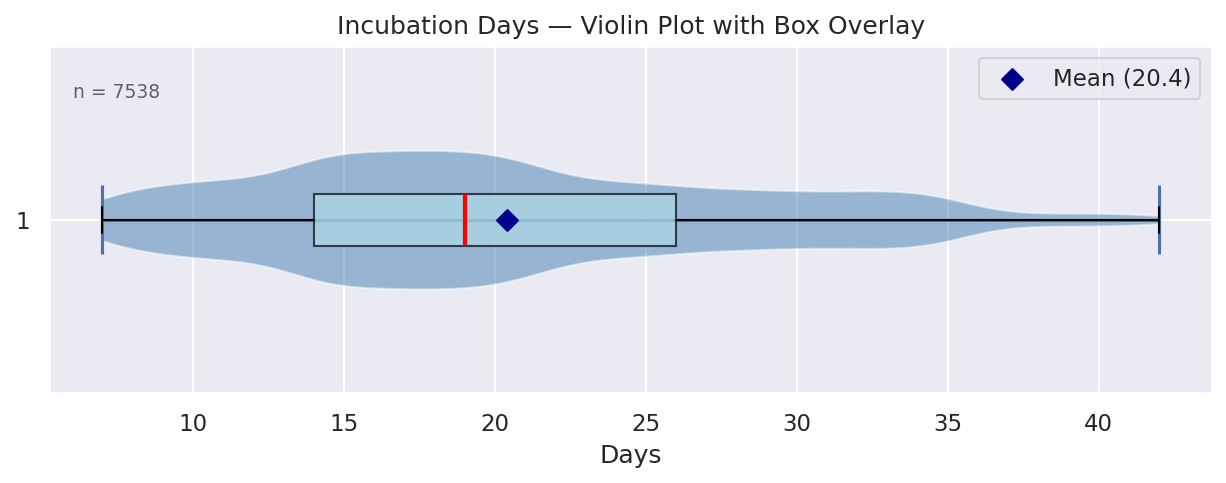
\includegraphics[width=0.85\textwidth]{incubation_violin.png}
\caption{Incubation days --- violin plot with box overlay. Mean (20.4) $>$ Median (19).}
\end{figure}

\begin{figure}[htbp]
\centering
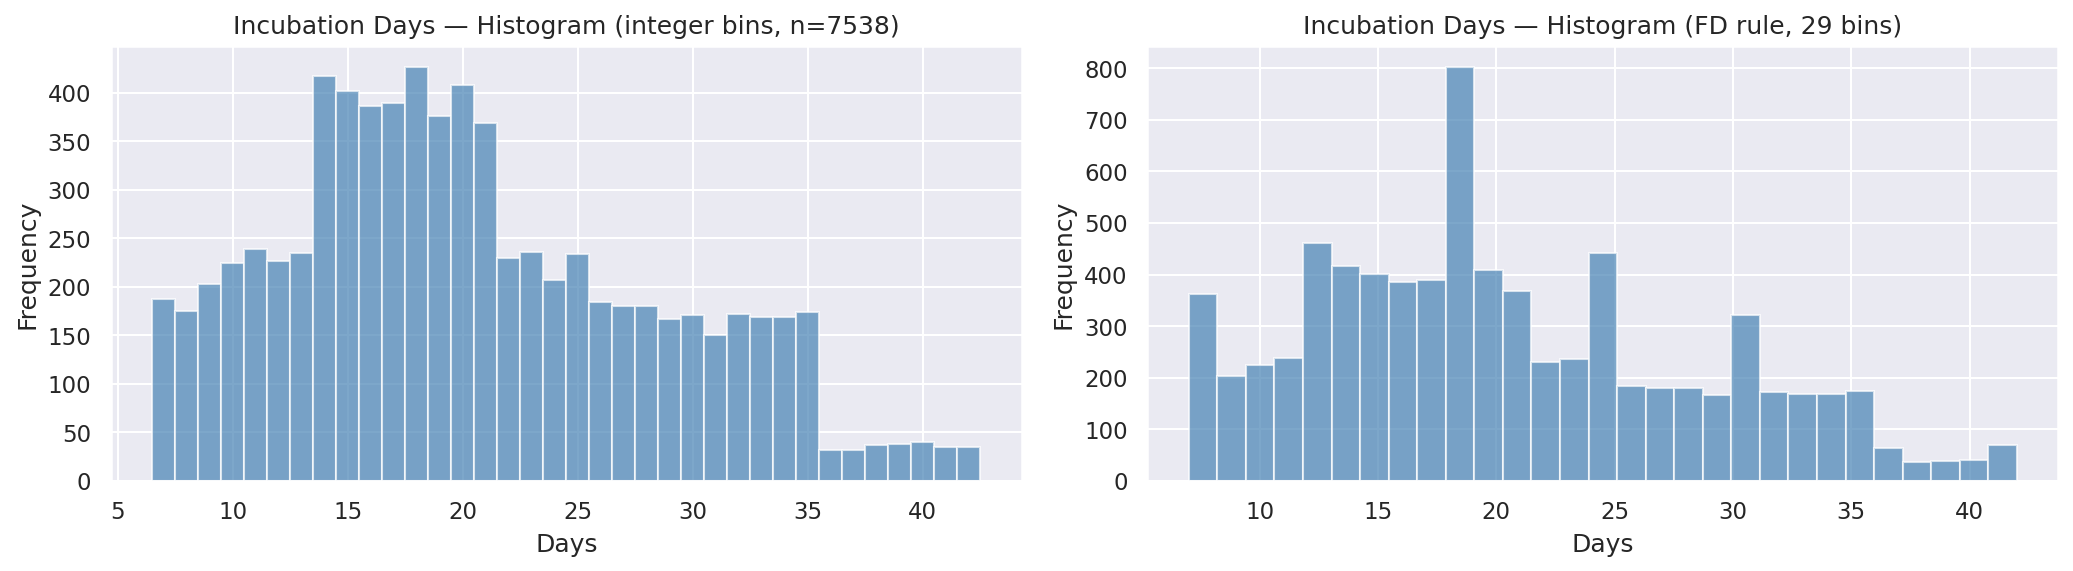
\includegraphics[width=0.85\textwidth]{incubation_histogram.png}
\caption{Incubation days --- integer-aligned bins (left) and FD-rule (right).}
\end{figure}

\begin{figure}[htbp]
\centering
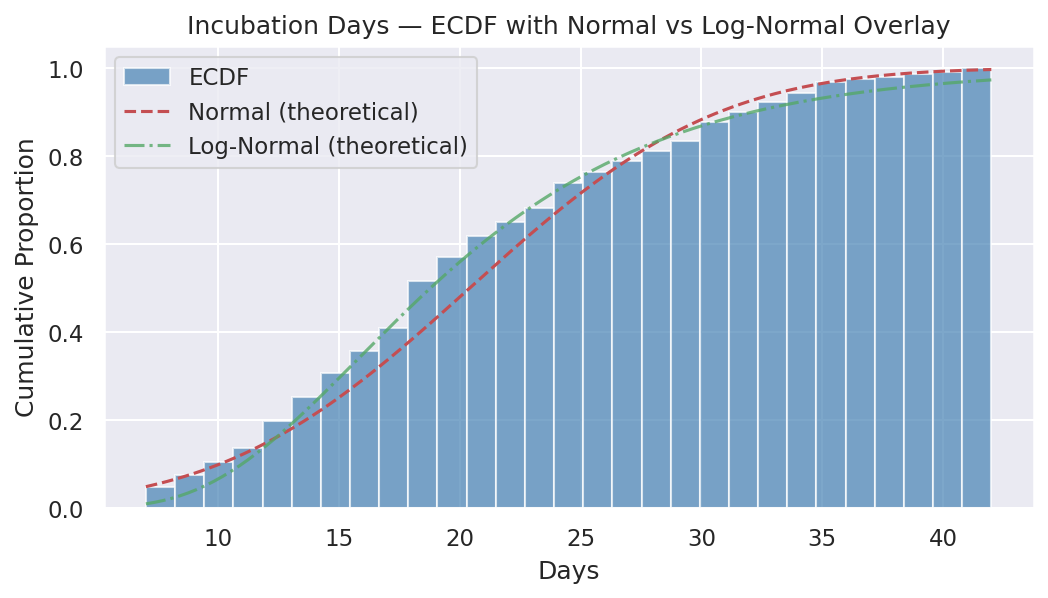
\includegraphics[width=0.7\textwidth]{incubation_ecdf.png}
\caption{Incubation days ECDF — the blue line deviates from normal (red dash), 
but follows the log-normal (green dash-dot) more closely.}
\end{figure}

\begin{figure}[htbp]
\centering
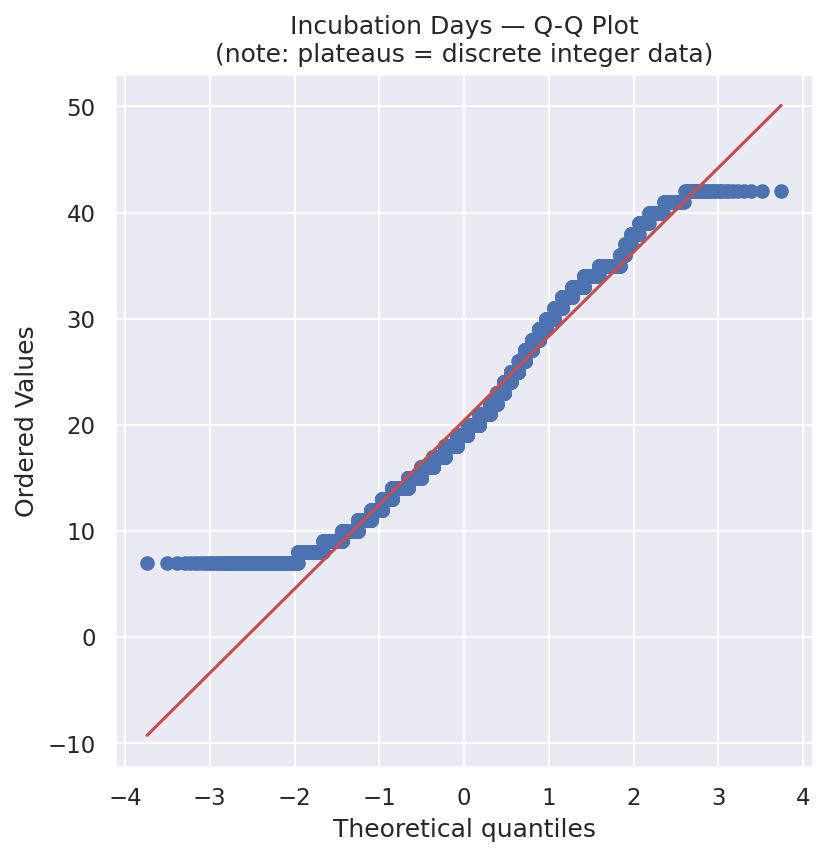
\includegraphics[width=0.55\textwidth]{incubation_qq.png}
\caption{Incubation days Q-Q plot. Points curve away from the diagonal at extremes.}
\end{figure}

\textbf{Questionnaire result:}
\begin{itemize}
\item User observed: right-skewed, thin tail, mean $>$ median, not normal
\item Numbers: skew=0.47, kurtosis=-0.49 (lighter tails + flatter peak than normal), mean=20.4 vs median=19
\item Shapiro-Wilk: p $\approx$ 0.000 — but n=7538 exceeds the reliable range. For n $>$ 5000, any trivial deviation yields p $<$ 0.001. Better: rely on |skew|$<$0.5 and visual ECDF/Q-Q assessment.
\item \textbf{Center:} Median (19d) --- skew is moderate but present
\item \textbf{Spread:} IQR (12d) or MAD (5d) --- std (8.1d) assumes symmetry
\end{itemize}

\newpage

\subsection{D2: Hospital Days (\texttt{D2\_hospital\_days.py, D2b\_hospital\_investigation.py})}

\subsubsection*{The Bimodal Discovery}

The overall histogram of hospital\_days appeared bimodal with dips at days 4 and 9.

\begin{figure}[htbp]
\centering
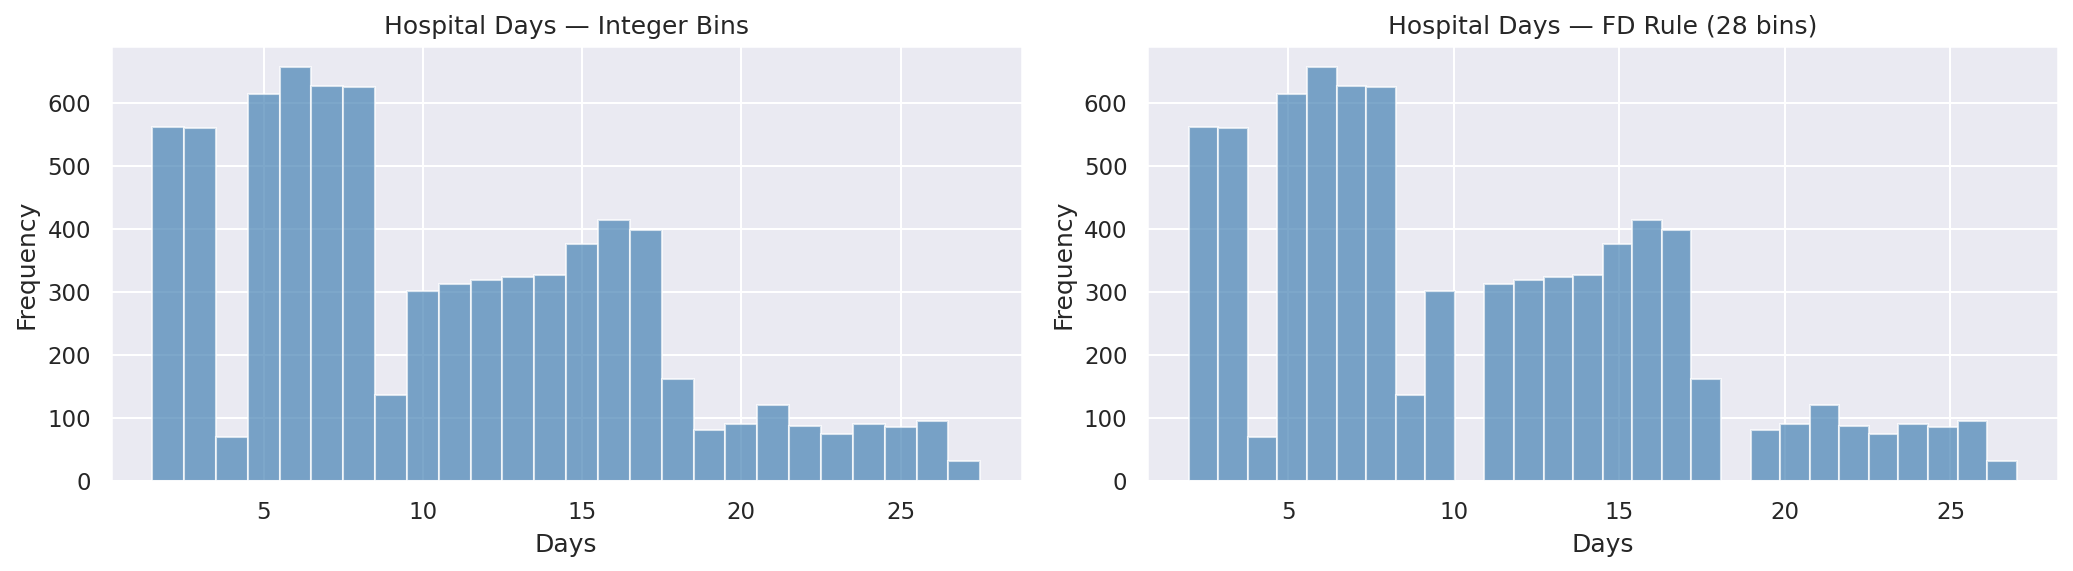
\includegraphics[width=0.85\textwidth]{hospital_histogram.png}
\caption{Hospital days histogram --- appears bimodal with dips at days 4 and 9.}
\end{figure}

We investigated four possible explanations (D2b):

\begin{table}[htbp]
\centering
\resizebox{\textwidth}{!}{
\begin{table}[htbp]
\caption{Hospital days stratified by severity level — each group has a distinct, non-overlapping center}
\label{tab:hospital_severity}
\begin{tabular}{lrllll}
\toprule
Severity & n & Mean & Median & Std & IQR \\
\midrule
Mild & 1121 & 2.5 & 2 & 0.5 & 1.0 \\
Moderate & 2669 & 6.5 & 6 & 1.2 & 3.0 \\
Severe & 2606 & 13.5 & 13 & 2.4 & 5.0 \\
Critical & 1142 & 20.6 & 21 & 3.6 & 7.0 \\
\bottomrule
\end{tabular}
\end{table}

}
\end{table}

\textbf{Conclusion:} Severity explains it perfectly. Each level has a distinct,
non-overlapping center. The "bimodal" shape is an \textbf{aggregation artifact}
mixing four unimodal distributions.

Other factors tested and ruled out:
\begin{itemize}
\item Outcome: weak effect (tracks severity naturally)
\item Syndrome: HPS vs HFRS nearly identical (10.3 vs 10.5 days)
\item Age group: all $\sim$10.4 days --- no effect
\end{itemize}

\textbf{Decision:} Do NOT smooth the histogram. The bumps are real signal.

\begin{figure}[htbp]
\centering

\includegraphics[width=0.85\textwidth]{hospital_by_severity.png}
\caption{Hospital days by severity --- each group is cleanly separated.}
\end{figure}

\newpage

\subsection{D3: ICU Days (\texttt{D3\_icu\_days.py, D3b\_icu\_investigation.py})}

\subsubsection*{Spike-and-Slab Distribution}

50.3\% of patients have icu\_days = 0. The minimum stay for admitted patients is 3 days.
ICU admission is perfectly predicted by severity:

\begin{table}[htbp]
\centering
\resizebox{\textwidth}{!}{
\begin{table}[htbp]
\caption{ICU admission rates and stay lengths by severity}
\label{tab:icu_severity}
\begin{tabular}{lrlll}
\toprule
Severity & n & ICU Rate & ICU Days (median) & ICU Days (mean) \\
\midrule
Mild & 1121 & 0\% & — & — \\
Moderate & 2669 & 0\% & — & — \\
Severe & 2606 & 100\% & 4 & 4.5 \\
Critical & 1142 & 100\% & 12 & 11.5 \\
\bottomrule
\end{tabular}
\end{table}

}
\end{table}

\begin{figure}[htbp]
\centering
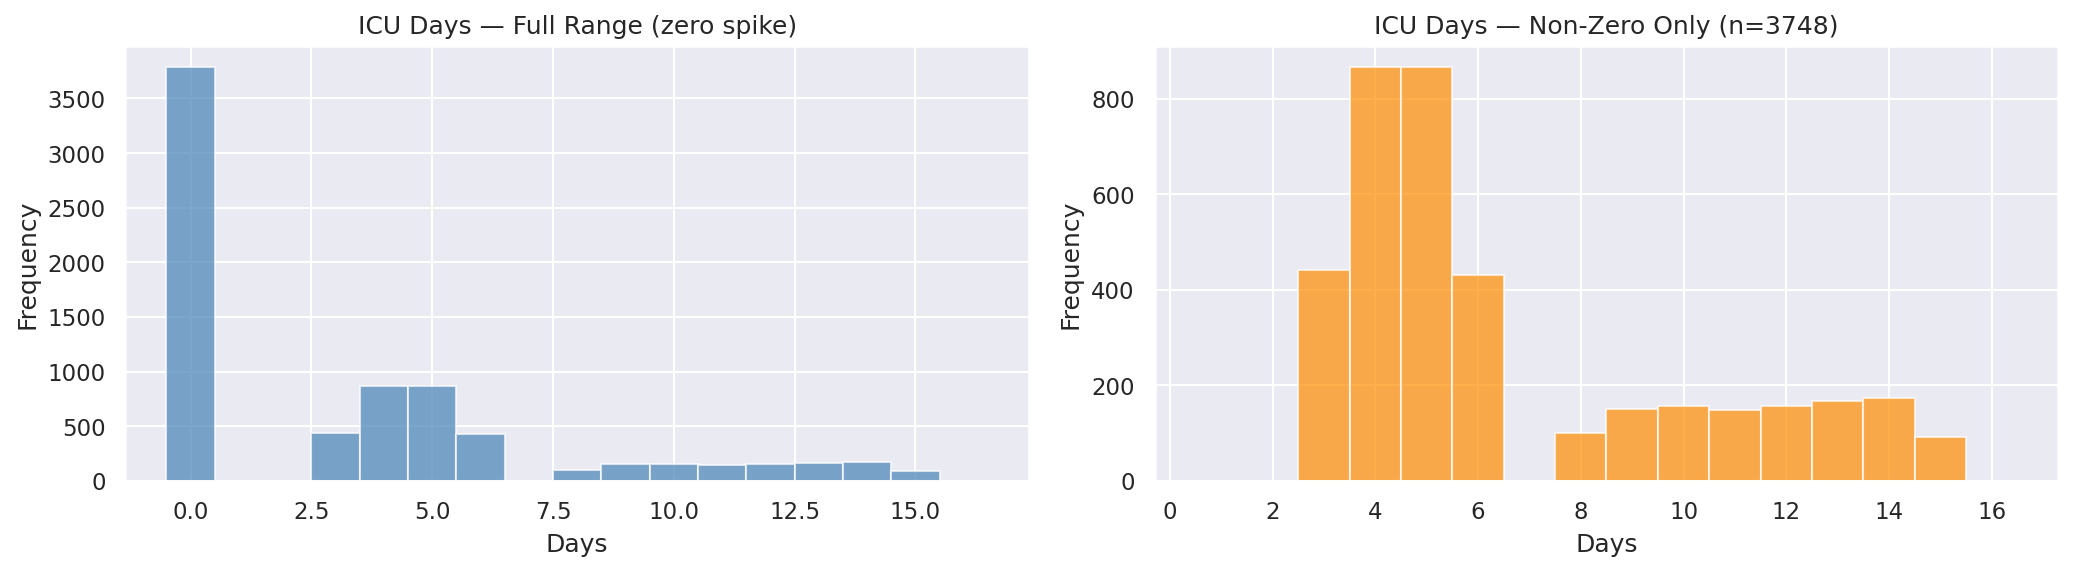
\includegraphics[width=0.85\textwidth]{icu_histogram.png}
\caption{ICU days --- massive zero spike (left). Non-zero only distribution (right).}
\end{figure}

\textbf{Decision:} Split into two separate questions --- (1) Who goes to ICU? (binary),
(2) How long do admitted patients stay? (continuous, non-zero only).

\subsection{D4: Average Temperature (\texttt{D4\_avg\_temp\_c.py})}

First near-normal variable. Skew=-0.15, mean$\approx$median.

\begin{figure}[htbp]
\centering
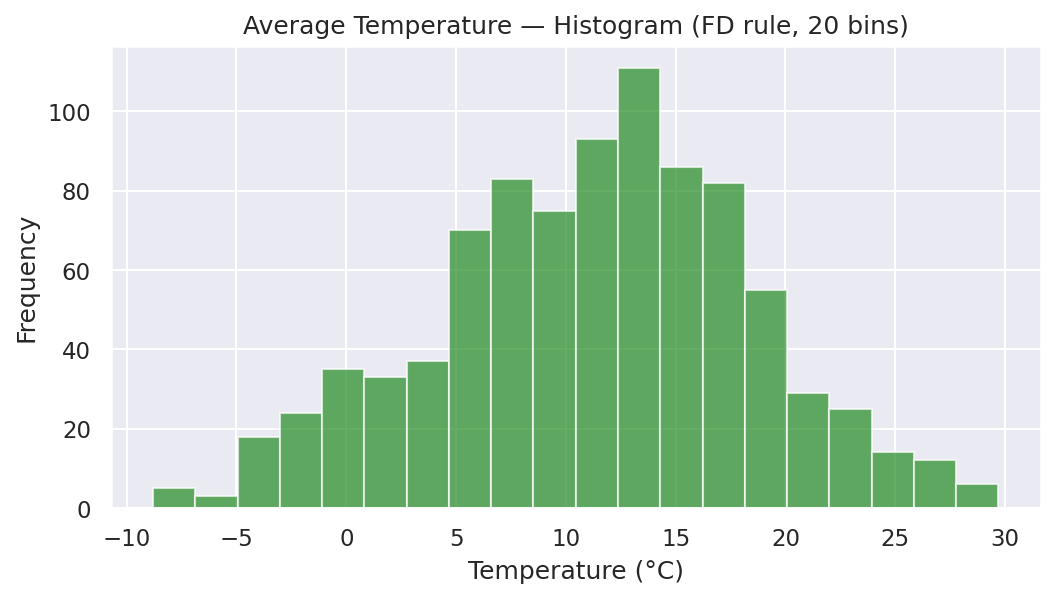
\includegraphics[width=0.85\textwidth]{temp_histogram.png}
\caption{Temperature --- approximately normal distribution.}
\end{figure}

\begin{figure}[htbp]
\centering
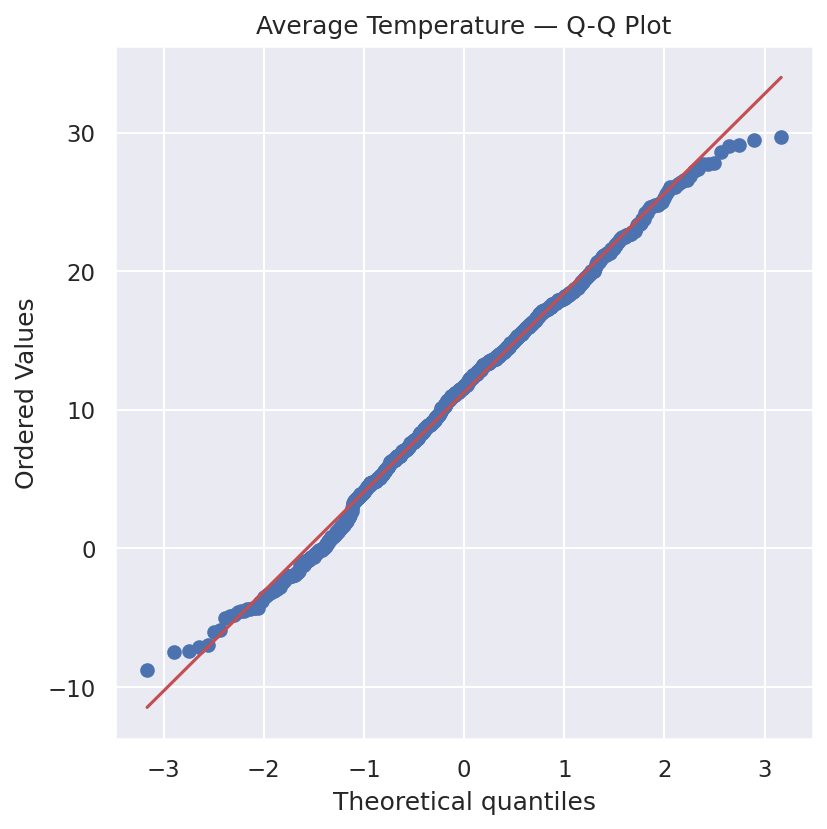
\includegraphics[width=0.7\textwidth]{temp_qq.png}
\caption{Temperature Q-Q plot --- follows the diagonal closely (nearly normal).}
\end{figure}

Only outlier: -8.8$^{\circ}$C in Ostrobothnia, Finland (real, kept).

\textbf{Lesson:} This is what a normal distribution looks like --- useful reference
for comparing with the skewed variables.

\newpage

\subsection{D5: Rainfall (\texttt{D5\_rainfall\_mm.py})}

Right-skewed (skew=1.80), heavy-tailed (kurtosis=5.05). Mean=253mm, Median=195mm.
Biome explains most variation.

\begin{figure}[htbp]
\centering
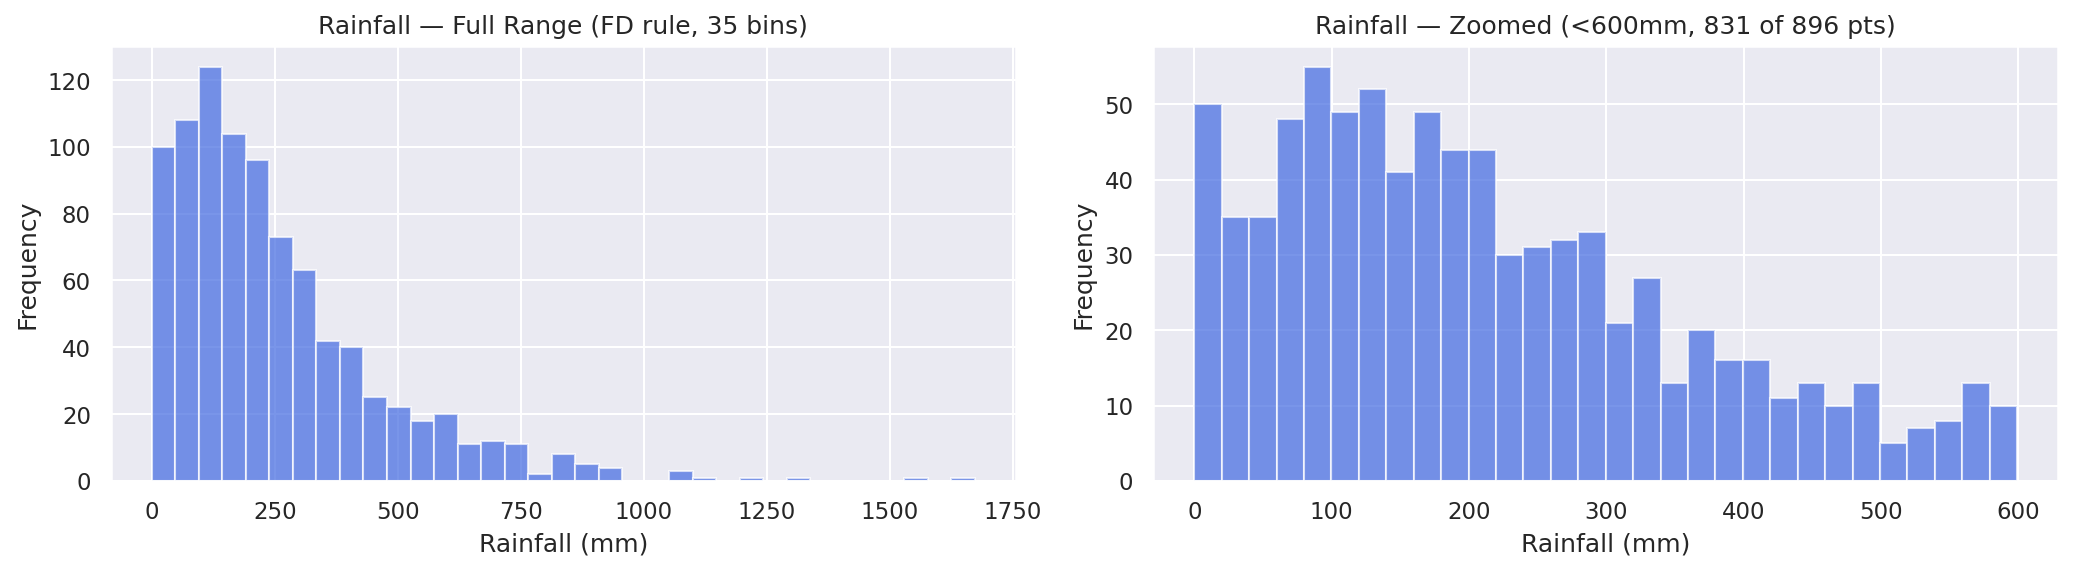
\includegraphics[width=0.85\textwidth]{rain_histogram.png}
\caption{Rainfall --- full range (left) and zoomed to $<$600mm (right).}
\end{figure}

\subsection{D6: Rodent Abundance (\texttt{D6\_rodent\_abundance.py})}

Most symmetric variable (skew=0.02). Bounded [0,1] but nearly identical across all 14 biomes
(range 0.64--0.72). Unlike rainfall (10x biome variation), rodent abundance is
constant --- suggesting local factors matter more than climate.
\textbf{Caveat:} This assumes comparable sampling protocols (trap effort, survey area) across biomes.
If methods differed, the apparent constancy could partly reflect methodological consistency.

\subsection{D7: Confirmed Cases (\texttt{D7\_confirmed\_cases.py})}

Most extreme skew: mean=1793, median=58 (31x gap!). Skew=2.82, kurtosis=7.14.

Top 20 highest case years are all China HFRS (17k--24k/year since 1970s).

\begin{figure}[htbp]
\centering
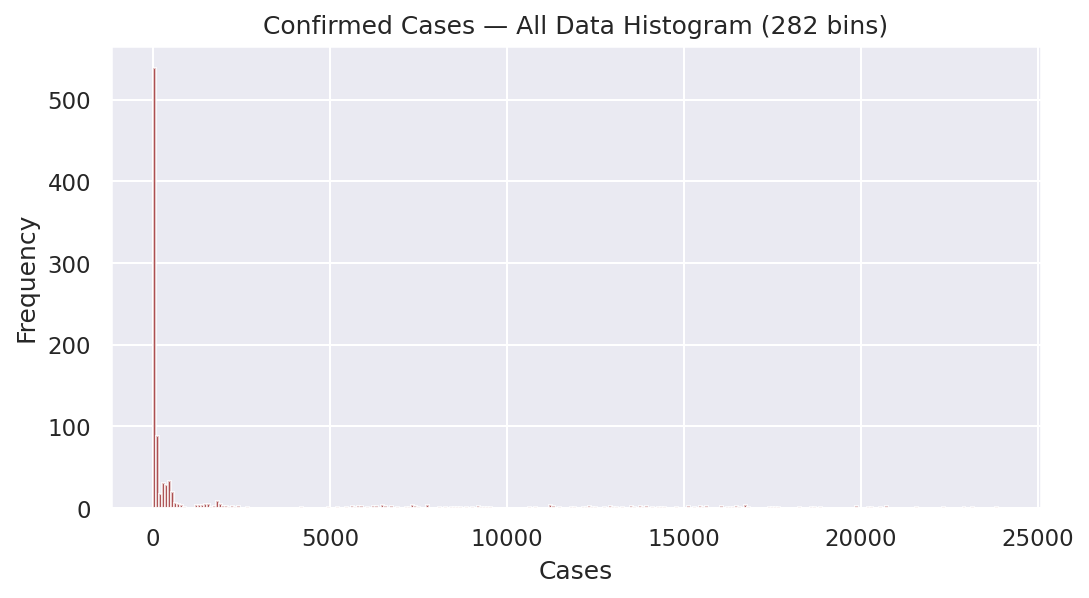
\includegraphics[width=0.85\textwidth]{cases_histogram.png}
\caption{Confirmed cases --- full range (left, massive tail) and zoomed (right, bulk of data).}
\end{figure}

\begin{figure}[htbp]
\centering
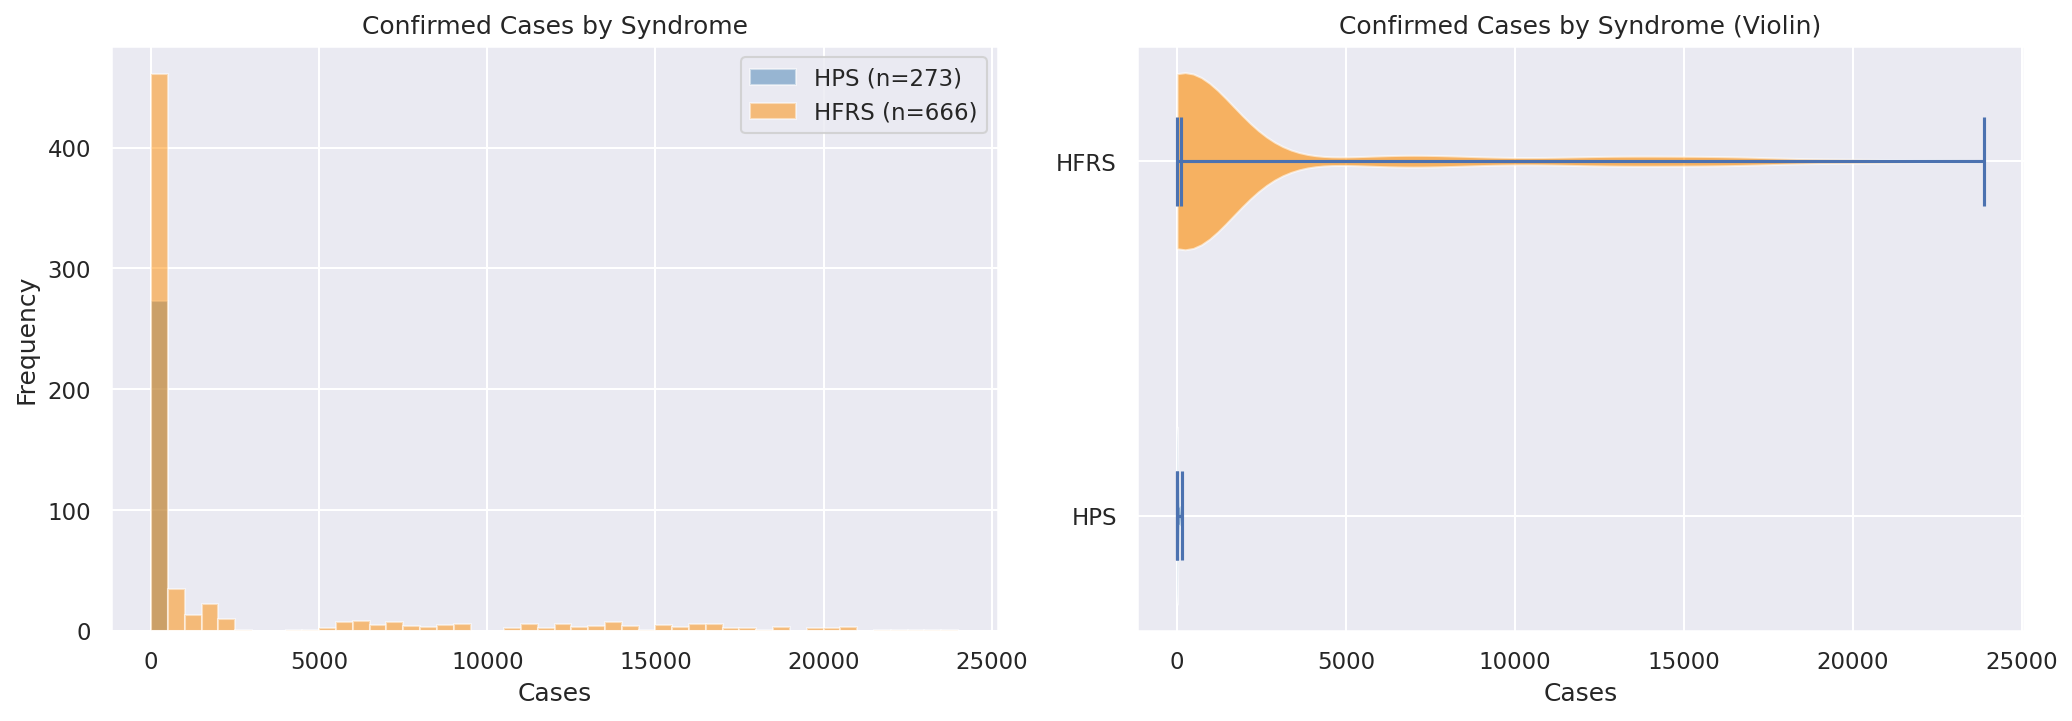
\includegraphics[width=0.65\textwidth]{cases_by_syndrome.png}
\caption{Confirmed cases by syndrome --- HPS vs HFRS. HFRS dominates.}
\end{figure}

\subsubsection*{The Underreporting Question}
Is the 100x difference between AMRO (mean=30) and WPRO (mean=5358) real?
Consistent data across decades and multiple countries supports real biological differences
in transmission ecology (rodent host distribution).

\begin{figure}[htbp]
\centering
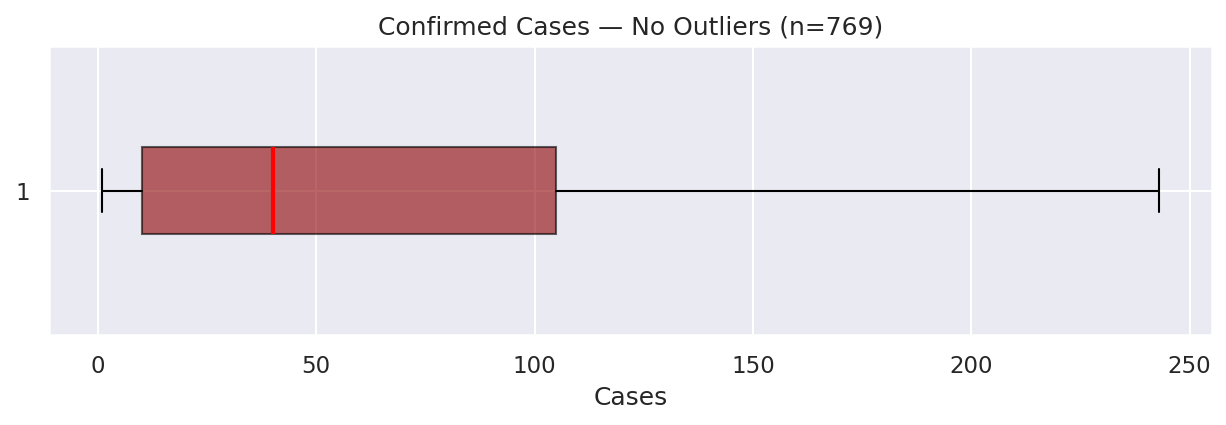
\includegraphics[width=0.85\textwidth]{cases_nooutliers_boxplot.png}
\caption{Confirmed cases --- no-outliers version (IQR-filtered, 170 points removed).}
\end{figure}

\newpage

\subsection{D8: Case Fatality Rate (\texttt{D8\_cfr.py})}

Bimodal by syndrome. HPS (mean=28.1\%) is 20x more lethal than HFRS (mean=1.4\%).

\begin{table}[htbp]
\centering
\resizebox{\textwidth}{!}{
\begin{table}[htbp]
\caption{Case fatality rate by syndrome — HPS is ~20x more lethal than HFRS}
\label{tab:cfr_syndrome}
\begin{tabular}{lrllll}
\toprule
Syndrome & n & Mean CFR & Median CFR & Max CFR & IQR \\
\midrule
HPS & 273 & 28.1\% & 29.0\% & 46.2\% & 12.3\% \\
HFRS & 666 & 1.4\% & 0.6\% & 6.5\% & 2.9\% \\
\bottomrule
\end{tabular}
\end{table}

}
\end{table}

\begin{figure}[htbp]
\centering
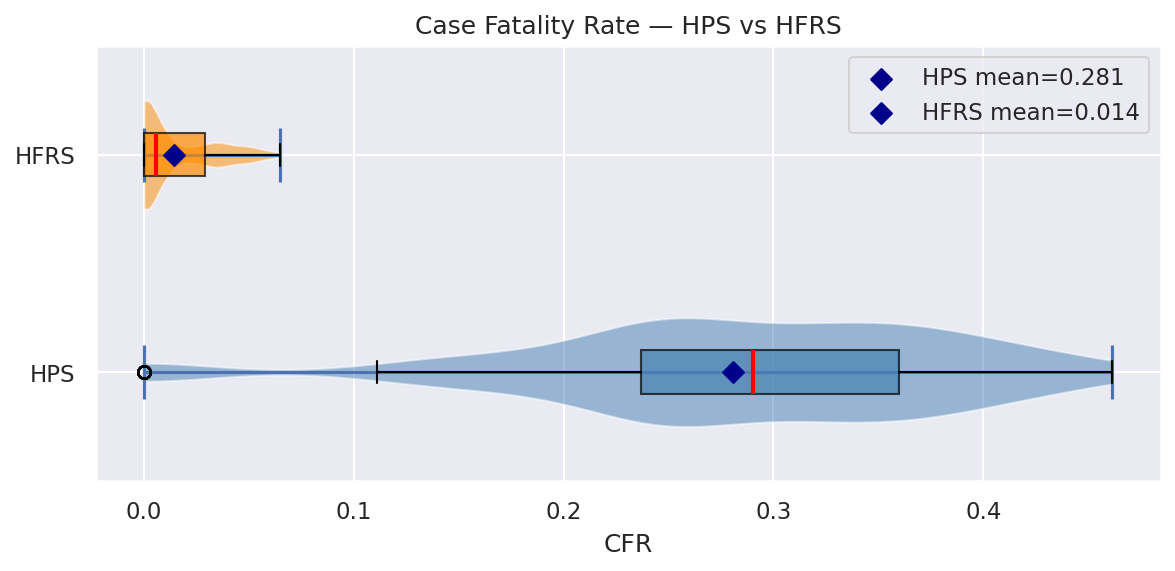
\includegraphics[width=0.8\textwidth]{cfr_combined.png}
\caption{Case fatality rate --- HPS vs HFRS side by side. The distributions barely overlap.}
\end{figure}

\textbf{Key insight:} The overall CFR (9.2\%) represents neither group. Never report
CFR as a single number for diseases with different syndromes.
\textbf{Note:} CFR differences may partly reflect healthcare access or time-to-treatment,
not just virology. If variables for these existed, stratifying by them would strengthen
the analysis.

\newpage

\section{Phase E: Comparative Analysis}

\subsection{E1 -- Comparative Violins (\texttt{E1\_comparative\_violins.py})}

\begin{figure}[htbp]
\centering

\includegraphics[width=0.85\textwidth]{compare_incubation_severity.png}
\caption{Incubation days by severity --- surprisingly similar across all four levels.}
\end{figure}

\begin{figure}[htbp]
\centering

\includegraphics[width=0.85\textwidth]{compare_incubation_syndrome.png}
\caption{Incubation days by syndrome --- HPS (16d) shorter than HFRS (22d).}
\end{figure}

\begin{figure}[htbp]
\centering

\includegraphics[width=0.85\textwidth]{compare_hospital_severity.png}
\caption{Hospital days by severity --- clean separation.}
\end{figure}

\begin{figure}[htbp]
\centering

\includegraphics[width=0.85\textwidth]{compare_temp_biome.png}
\caption{Temperature by biome, sorted coldest to warmest.}
\end{figure}

\begin{figure}[htbp]
\centering

\includegraphics[width=0.85\textwidth]{compare_rain_biome.png}
\caption{Rainfall by biome, sorted driest to wettest. Desert (63mm) to Valdivian forest (630mm).}
\end{figure}

Sample size labels (n=...) are shown on each violin. For any subgroup with n $<$ 30,
violin KDE becomes unstable and a box-only plot should be used instead.

\newpage

\subsection{E2 -- Bar Chart Critique (\texttt{E2\_bar\_chart\_critique.py})}

\begin{figure}[htbp]
\centering

\includegraphics[width=\textwidth]{critique_bar_vs_violin.png}
\caption{Side-by-side comparison: bar chart + error bars (left) vs violin + box (right).}
\end{figure}

The bar chart (left) looks clean, but hides:
\begin{enumerate}
\item \textbf{Sample size:} n=1121 vs n=1142 --- same bar, different reliability
\item \textbf{Distribution shape:} Each group has a different shape (tight, spread, skewed)
\item \textbf{Multimodality:} If a group were bimodal, you'd never know
\item \textbf{Outliers:} Hidden completely
\item \textbf{Mean assumption:} Error bar assumes symmetric normal --- hospital\_days violates this
\end{enumerate}

The violin + box (right) conveys: n, min, Q1, median, Q3, max, shape, skew, tails.

\textbf{Bottom line:} Bar charts are not "cleaner." They are less honest.

\newpage

\section{Master Summary Table}

\begin{table}[htbp]
\centering
\resizebox{\textwidth}{!}{
\begin{table}[htbp]
\caption{Summary statistics for all numeric variables across datasets}
\label{tab:master}
\begin{tabular}{lrlllllllll}
\toprule
Variable & n & Mean & Median & Std & IQR & MAD & Skewness & Kurtosis & Best Center & Best Spread \\
\midrule
Incubation Days & 7538 & 20.41 & 19.00 & 8.07 & 12.00 & 5.00 & 0.47 & -0.49 & Mean & Std \\
Hospital Days & 7538 & 10.46 & 9.00 & 6.18 & 9.00 & 4.00 & 0.60 & -0.42 & Median & Iqr \\
ICU Days & 7538 & 3.30 & 0.00 & 4.16 & 5.00 & 0.00 & 1.19 & 0.50 & Median & Iqr \\
Temperature (°C) & 896 & 11.26 & 11.70 & 7.18 & 9.70 & 4.90 & -0.15 & -0.25 & Mean & Std \\
Rainfall (mm) & 896 & 252.83 & 195.35 & 217.76 & 237.10 & 108.60 & 1.80 & 5.05 & Median & Iqr \\
Rodent Abundance & 896 & 0.67 & 0.67 & 0.18 & 0.30 & 0.15 & 0.02 & -1.12 & Mean & Std \\
Confirmed Cases & 939 & 1792.77 & 58.00 & 4470.37 & 415.00 & 51.00 & 2.82 & 7.14 & Median & Iqr \\
Case Fatality Rate & 939 & 0.09 & 0.02 & 0.13 & 0.17 & 0.02 & 1.28 & 0.08 & Median & Iqr \\
\bottomrule
\end{tabular}
\end{table}

}
\end{table}

\textbf{Decision guide:} For symmetric variables (temperature, rodent abundance), mean + std
is appropriate. For skewed variables (incubation, rainfall, cases), median + IQR is honest.
For spike-and-slab (ICU), report separately. For bimodal (CFR), report per syndrome.

\section{Key Lessons}

\subsection{Statistical}
\begin{enumerate}
\item Mean vs median gap is the quickest asymmetry test
\item For skewed data: median + IQR; for symmetric: mean + std
\item Kurtosis reveals tail behavior independent of skew
\item Shapiro-Wilk is unreliable for n $>$ 5000
\item Small n (outbreaks: 20) produces unreliable estimates
\end{enumerate}

\subsection{Visualization}
\begin{enumerate}
\item KDE and Q-Q assume continuous data --- misbehave on discrete/bounded
\item Integer data needs integer-aligned bins, not sqrt rule
\item ECDF with theoretical normal overlay is more robust than Q-Q for bounded data
\item Violin + box conveys more information than bar + error bar
\item Always check subgroups before describing shape
\item Provide both full-range and no-outliers versions for skewed data
\end{enumerate}

\subsection{Epidemiological}
\begin{enumerate}
\item Incubation is similar across severity but differs by syndrome (HPS shorter)
\item Hospital/ICU stays differ by severity with clean separation
\item HPS (28.1\% CFR) is 20x more lethal than HFRS (1.4\% CFR)
\item China HFRS drives the extreme tail in confirmed cases
\item Rodent abundance is constant across biomes; rainfall varies 10x
\end{enumerate}

\end{document}
